% !TeX spellcheck = ru_RU-Russian
\documentclass[utf8,12pt]{jetp}
%\twocolumn

\def\baselinestratch{1.5}

\DeclareMathOperator{\arcsh}{arcsh}
\DeclareMathOperator{\arcch}{arcch}
\DeclareMathOperator{\Det}{Det}
\DeclareMathOperator{\Cl}{Cl}
\DeclareMathOperator{\Li}{Li}
\DeclareMathOperator{\im}{Im}

\DeclareUnicodeCharacter{2212}{\textendash}

\begin{document}

\title{Обобщенная модель Изинга на квадратной решетке}
	
\setaffiliation1{Российский федеральный ядерный центр --- ВНИИТФ им. академика Е. И. Забабахина, 456770, Снежинск, Челябинская обл., Россия} %
\setaffiliation2{Институт физики металлов им. М. Н. Михеева  Уральского отделения Российской академии наук \\ 620108, Екатеринбург, Россия}
	
\setauthor{Е.~С.}{Цуварев}{12}
\email{eguny@mail.ru}
	
\setauthor{Ф.~А.}{Кассан-Оглы}{2}
\email{felix.kassan-ogly@imp.uran.ru}

	
\rtitle{Обобщенная модель Изинга на квадратной решетке}
\rauthor{Е.~С.~Цуварев, Ф.~А.~Кассан-Оглы}
	
	
\abstract{Впервые получено точное аналитическое решение обобщенной модели Изинга на квадратной решетке комбинаторным методом Вдовиченко--Фейнмана. Исследованы термодинамические и магнитные свойства обобщенной модели Изинга на квадратной решетке с двумя трансляциями в горизонтальном и вертикальном направлениях. Установлены новые особенности, возникающие в обобщенной модели Изинга.}
	
\maketitle

\section{Введение}

В текущем календарном году исполняется ровно сто лет со времени опубликования исходной статьи по классической модели Изинга на линейной регулярной одноатомной цепочке спинов с двумя состояниями в присутствии внешнего магнитного поля и с обменным взаимодействием только между ближайшими соседями Эрнстом Изингом в журнале Zeitschrift für Physik под названием Beitrag zur Theorie des Ferromagnetismus~\cite{ising1925}. Изинг произвел детальный точный расчет свободной энергии Гельмгольца и продемонстрировал, что при обозначенных условиях не наблюдается никакого фазового перехода ни при какой конечной температуре. На основе полученных результатов он сделал заключение, что в рассматриваемой модели не может быть фазового перехода при любых размерностях.

Однако в 1936 году Рудольф Пайерлс опубликовал статью~\cite{peierls1936}, в которой вопреки утверждению Изинга, он доказал, что модель Изинга должна испытывать переход в 2D и 3D случаях. В 1941 году Крамерс и Ваннье при сопоставлении низкотемпературного и высокотемпературного разложения статистической суммы и с помощью изобретенного ими дуального превращения вычислили критическую температуру фазового перехода в модели Изинга на квадратной решетке с обменным взаимодействием между ближайшими соседями по горизонтальному и вертикальному направлению~\cite{kramers_wannier1, kramers_wannier2}.

Впоследствии в 1944 году~\cite{onsager1941} Онзагер, используя метод трансфер-матрицы Крамерса-Ваннье весьма сложным методом, основанным на алгебрах Ли, получил точное аналитическое решение для свободной энергии Гельмгольца в модели Изинга на квадратной решетке. Эта работа открыла новую эпоху и фактически определила границу размежевания между предыдущими наивными, весьма упрощенными теориями типа молекулярного поля и современной эрой исследования критических явлений в статистической физике с сопутствующими особенностями поведения термодинамических величин. 

Труднопреодолимость весьма сложного оригинального метода Онзагера, а, главное, выдающийся результат Онзагера побудил многих высококлассных исследователей, как физиков, так и математиков, к поискам самых разнообразных направлений обобщений по разработке более простых и эффективных методов получения точных решений с одной стороны, а с другой стороны, к расширению объектов и задач исследований. Точное аналитическое решение для свободной энергии Гельмгольца в модели Изинга на квадратной решетке было успешно переполучено в разнообразных комбинаторных подходах, развитых, в частности, Кацем и Вардом~\cite{kac1952}, Поттсом и Вардом~\cite{potts1955}, Хёрстом и Грином~\cite{hurst1960}, Вдовиченко~\cite{vdovichenko1964, vdovichenko1965}, Фейнманом~\cite{feynman1972}, а в более поздних теориях, основанных на грассмановых переменных: Самуэлем~\cite{samuel1980}, Плечко~\cite{plechko1985}, а также с использованием алгебры Клиффорда-Дирака Вергелесом~\cite{vergeles2009}.

К настоящему времени, количество научных статей по модели Изинга исчисляется тысячами и тысячами, и продолжает только увеличиваться, не обнаруживая спада активности. Однако следует отметить, что, несмотря на огромные затраченные усилия, направленные на поиски точных решений для свободной энергии в ряде случаев оказались не решенными до сих пор. Во-первых, это невозможность обобщения на 3D объекты. Во-вторых, отсутствие решений во внешнем магнитном поле ни на одной из 2D решеток. В-третьих, точно установлено, что решениям поддаются не все 2D решетки, а только лишь планарные, то есть те, в которых отсутствуют пересечения между обменными взаимодействиями. В-четвертых, модель Изинга при обобщении на спины с числом состояний более двух также не поддается точному решению. 

Ввиду указанных непреодолимых препятствий на пути более углубленных исследований, интересы исследователей постепенно переключались на применение модели Изинга к более широким объектам, в частности, 2D планарным решеткам: к классу одиннадцати Архимедовых и классу дуальных Архимедовым восьми решеток Лавэ; подробное изложение свойств решеток этих классов и строгое доказательство их уникальности изложено в книге Грюнбаума и Шефарда~\cite{grunbaum1987}. 

К настоящему времени точные выводы свободной энергии Гельмгольца получены на многих Архимедовых  решетках, в том числе: на квадратной решетке Онзагером~\cite{onsager1941}, на треугольной решетке Ваннье~\cite{wannier1950}, на гексагональной решетке Гутаппелем~\cite{houtapell1950}, на решетке кагоме Кано и Найем~\cite{kano_naya1953}, на решетке баунс (ruby) Лином и Ма~\cite{lin1983}, на решетке кросс (решетка 4-6-12) Лином и Хуангом~\cite{lin1985}. 

Точные решения свободной энергии Гельмгольца в модели Изинга получены и на некоторых решетках Лавэ (которые являются дуальными Архимедовым  решеткам); среди них: Ваксом, Ларкиным и Овчинниковым на решетке Union Jack~\cite{vaks1965}, Урюмовым на решетке Cairo pentagonal~\cite{urumov2002}, Хольцером на Dice решетке~\cite{holzer1990}.

Существуют также точные выводы свободной энергии Гельмгольца на ряде решеток, не входящих ни в класс Архимедовых, ни в класс Лавэ, в частности, Лином и Вангом на одном типе решетки 4-6~\cite{lin1988}, Оитмаа и Кеппертом на другом типе решетки 4-6~\cite{oitmaa2002}, Стречкой и Кановой на решетке bow-tie~\cite{strecka2008}, Чао, Лии и Лином на решетке 3-6~\cite{chao1990}, а также Ло, Яо и Карлсоном на решетке TKL (triangular kagome lattice)~\cite{loh2008}.

Поскольку точному решению поддаются только планарные решетки, а даже учет взаимодействия между спинами на вторых соседях не отвечает условию планарности, то интерес исследователей переключился на новое направление, а именно, возникли множественные попытки решить задачу в случае только взаимодействий между ближайшими соседями, но разными между разными соседними спинами. Фактически это означает переход на более высокий уровень — исследование решеток с трансляциями на два периода решетки по всем направлениям. Строго говоря, на всех указанных выше решетках такая задача решается как бы компромиссным образом — число учитываемых взаимодействий больше, чем с трансляциями на один период решетки, но меньше, чем на два периода. 

В качестве примера рассмотрим историю исследования решетке Union Jack. Первоначально, Ваксом, Ларкиным и Овчинниковым~\cite{vaks1965} свободная энергия Гельмгольца выведена точно, при учете двух взаимодействий (исходная решетка с трансляциями на один период решетки по двум направлениям), затем Чикью и Сузуки~\cite{chikyu1987} сосчитали свободную энергию Гельмгольца с тремя обменными взаимодействиями, Морита~\cite{morita1986} обобщил задачу на четыре взаимодействия, и позднее Ву и Лином~\cite{wu1987} задача решена точно с учетом шести взаимодействий. И, тем не менее, окончательного решения не найдено, поскольку в решетке Union Jack с трансляциями на два периода решетки число обменных взаимодействий равно восьми. В итоге получается, что задача с трансляциями на два периода решетки до конца не решена ни на одной из решеток, кроме одной, а именно, на квадратной решетке, причем без какого либо вывода и исследования свойств полученного выражения, (см., например,~\cite{syozi1972, utiyama1951}).

Целями настоящей работы является вывод точного аналитического выражения для свободной энергии Гельмгольца в модели Изинга на квадратной решетке с трансляционной инвариантностью на два периода решетки в горизонтальном и вертикальном напрвлениях с использованием наиболее удобного и эффективного метода Вдовиченко-Фейнмана, а также исследование физических свойств полученного решения при произвольном варьировании величин и знаков четырех обменных взаимодействий.

\section{Вычисление свободной энергии комбинаторным методом}

Идея комбинаторного решения модели Изинга на двумерной решетке принадлежит Фейнману~\cite{feynmann1978}. Суть метода заключается в подсчете всех суперпозиций замкнутых многоугольников (не имеющих общих сторон) на двумерной решетке. В последствие, предположение Фейнмана развивалось в статьях Каца и Уорда~\cite{kac1952}, Монтролла~\cite{montroll1953} и Вдовиченко~\cite{vdovichenko1965}. Так или иначе, метод берет свое начало с высокотемпературного разложения статистической суммы двумерной решетки. 

В нашей предыдущей работе~\cite{generalizedIsing2021} была упомянута квадратная решетка с обобщением на две трансляции в горизонтальном и вертикальном направлениях, предложенное Сиози (рис.~\ref{gen}). В своих работах Сиози \cite{syozi1, syozi2} предложил формулу для расчета внутренней энергии (но без доказательства). В этой работе будет получено точное аналитическое решение обобщенной модели Изинга на квадратной решетке с помощью комбинаторного метода.

\begin{figure}[h]
	\center{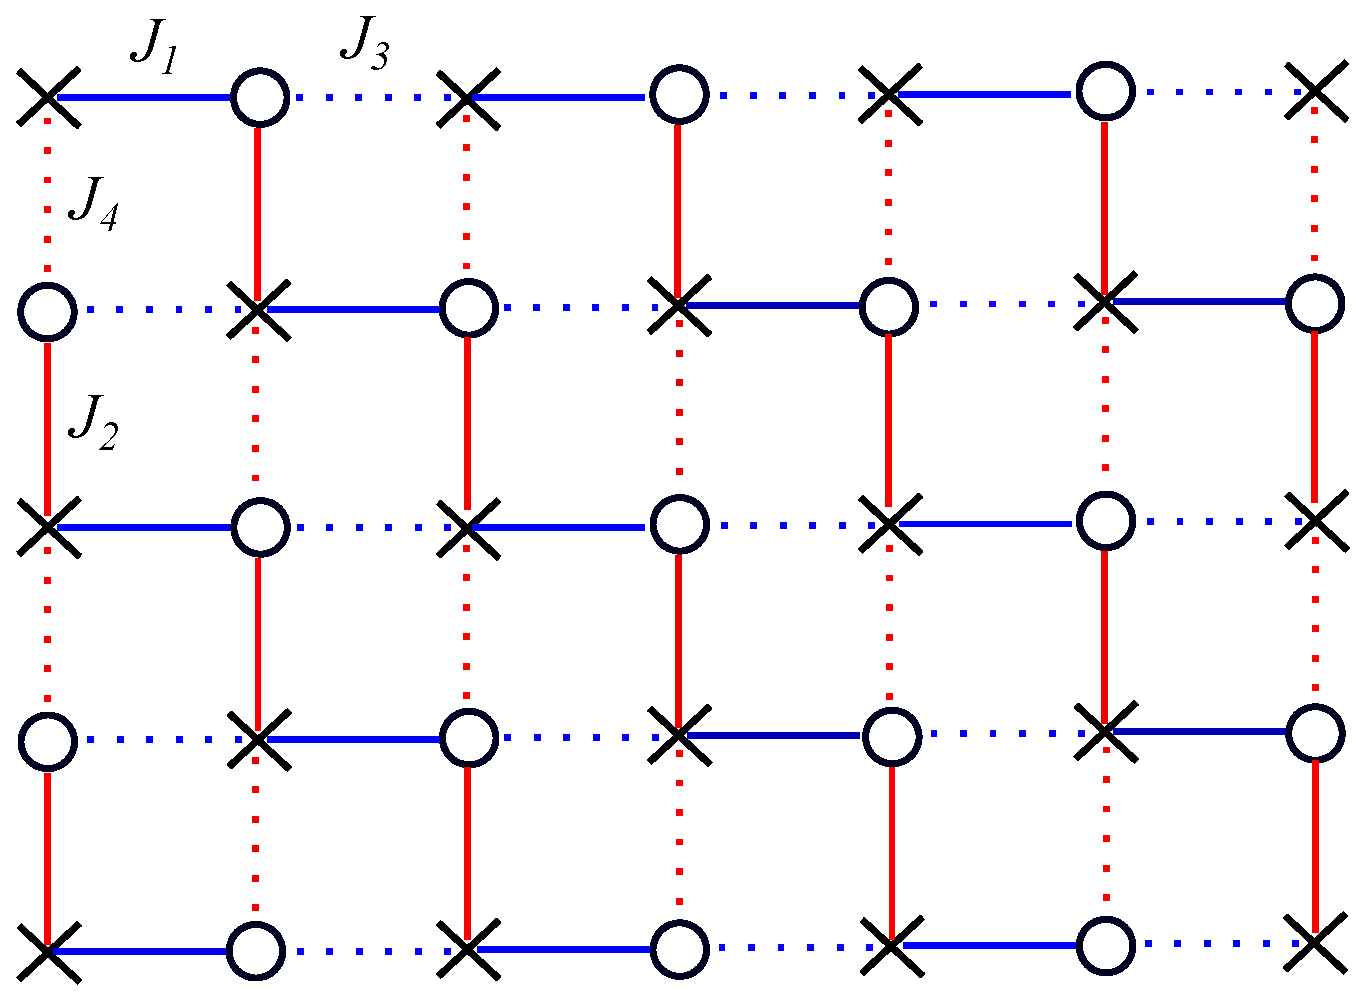
\includegraphics[width=0.6\linewidth]{Pictures/gen.eps}}
	\caption{Обобщенная квадратная решетка}
	\label{gen}
\end{figure}

Статсумму приведенной квадратной решетки (рис.~\ref{gen}) можно представить следующим образом 
\begin{equation}
Z_{N} = \sum_{\{\sigma\}} \exp{\bigg[ K_1 \sum_{\substack{i = 1,3,\dots \\ j = 2,4,\dots}} \sigma_i \sigma_j + K_2 \sum_{\substack{i = 2,4,\dots \\ k = 3,5,\dots}} \sigma_i \sigma_k + K_3 \sum_{\substack{i = 2,4,\dots \\ j = 3,5,\dots}} \sigma_i \sigma_j + K_4 \sum_{\substack{i = 1,3,\dots \\ k = 2,4,\dots}} \sigma_i \sigma_k\bigg]},
\end{equation}
где первая и третья суммы идут по половинам спинов в горизонтальном направлении,  а вторая и четвертая суммы идут по половинам спинов в вертикальном направлении, так что
\begin{equation*}
K_1 = \frac{J_1}{T}; \;\;\;\;\;\; K_2 = \frac{J_2}{T};\;\;\;\;\;\; K_3 = \frac{J_3}{T};\;\;\;\;\;\;K_4 = \frac{J_4}{T}.
\end{equation*}

Перепишем статсумму в виде
\begin{align}
&Z_{N} = (\ch K_1 \ch K_2 \ch K_3 \ch K_4)^N S, \nonumber \\
&S = \sum_{\{\sigma\}} \prod_{\substack{i = 1,3,\dots \\ j = 2,4,\dots}} (1 + v \sigma_i \sigma_j) \prod_{\substack{i = 2,4,\dots \\ k = 3,5,\dots}} (1 + u \sigma_i \sigma_k) \times \nonumber\\&\;\;\;\;\;\;\;\;\; \times \prod_{\substack{i = 2,4,\dots \\ j = 3,5,\dots}} (1 + w \sigma_i \sigma_j) \prod_{\substack{i = 1,3,\dots \\ k = 2,4,\dots}} (1 + t \sigma_i \sigma_k).
\label{z} 
\end{align}

Здесь $v = \th K_1$, $u = \th K_2$, $w = \th K_3$, $t = \th K_4$, а $N = L^2$ --- число спинов в решетке. Величина $S$ является полиномом от $v$, $u$, $w$ и $t$, в котором коэффициент $g_{nmlk}$ при $v^n u^m w^l t^k$ равен количеству способов построения замкнутых многоугольников, при которых общее количество горизонтальных связей равно $n+l$, а общее количество вертикальных связей равно $m+k$.

В статье Вдовиченко~\cite{vdovichenko1965} было показано, что для модели Изинга на обычной квадратной решетки величина $g_{nm}$ может быть представлена в виде суммы по замкнутым циклам, причем каждый цикл берется с множителем $(-1)^s$, где $s$ --- количество самопересечений замкнутого многоугольника. Наш случай ни сколько не отличается от обычного, за исключением того, что на обобщенной квадратной решетке встречаются два вида узлов (рисунок \ref{point}) (см. статьи~\cite{vaks1966, chikyu1987}). У узла, помеченного крестом (рисунок \ref{point}а), связь между соседним верхним узлом с обменным взаимодействием $J_2$, между соседним нижним узлом --- $J_4$, между соседним левым узлом --- $J_3$, между соседним левым узлом --- $J_1$. У узла, обозначенного кружком (рисунок \ref{point}б), наоборот: связь между соседним верхним узлом с обменным взаимодействием $J_4$, между соседним нижним узлом --- $J_2$, между соседним левым узлом --- $J_1$, между соседним левым узлом --- $J_3$. 

\begin{figure}[h]
	\begin{minipage}[h]{0.4\linewidth}
		\center{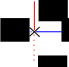
\includegraphics[width=0.7\linewidth]{Pictures/point1.eps} \\ а)}
	\end{minipage}
	\hfill
	\begin{minipage}[h]{0.4\linewidth}
		\center{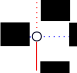
\includegraphics[width=0.7\linewidth]{Pictures/point2.eps} \\ б)}
	\end{minipage}
	\caption{Два вида узлов на обобщенной квадратной решетке }
	\label{point}
\end{figure}

В связи с этим, в отличие от обычной квадратной решетки, имеем 8 различных направлений на обобщенной квадратной решетке (рисунок \ref{dirgen}): 4 направления из узла , обозначенного кружком (вверх, вниз, влево, вправо) и 4 направления из узла, обозначенного крестом (вверх, вниз, влево, вправо).

\begin{figure}[h]
	\center{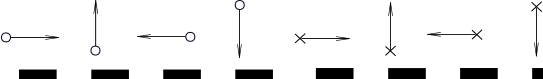
\includegraphics[width=0.9\linewidth]{Pictures/dirgen.eps}}
	\caption{Возможные направления на обобщенной квадратной решетке}
	\label{dirgen}
\end{figure}

Так же как и в случае обычной квадратной решетки, введем матрицу коэффициентов $\Lambda$, рекурсивные уравнения можно записать в виде
\begin{equation}
W_{r+1}(i, j, \mu) = \sum_{i^{'},\; j^{'},\; \mu^{'}} \Lambda (ij\mu\; |\; i^{'}j^{'}\mu^{'}) W_{r} (i^{'}, j^{'}, \mu^{'}),
\end{equation}

Поскольку существует восемь возможных направлений для движения по решетке, $\Lambda$ представляет собой матрицу $8 \times 8$ с индексами $\mu^{'}$ и $\mu$, графическая интерпретация которой показана на рисунке \ref{matxgen}. 

\begin{figure}[h]
	\center{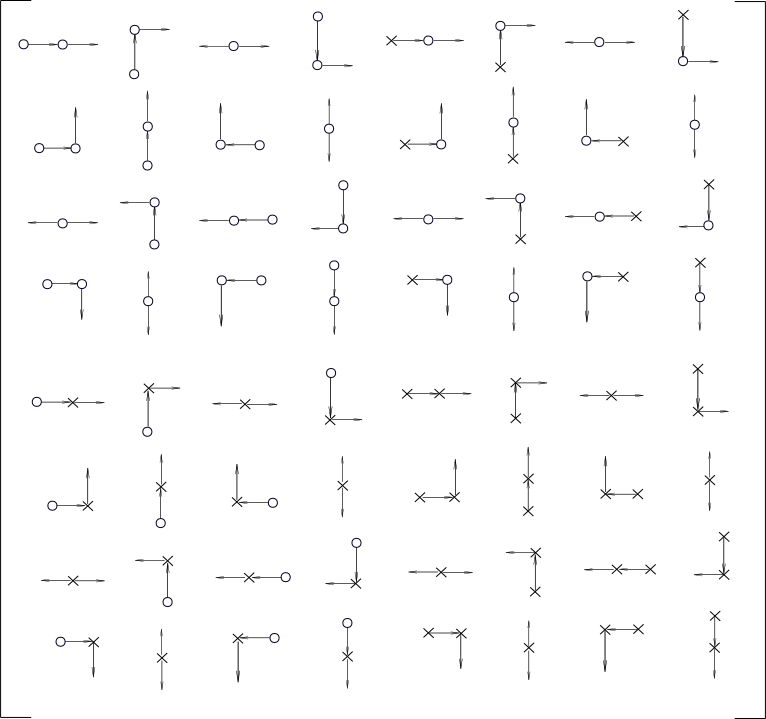
\includegraphics[width=0.7\linewidth]{Pictures/matxgen.eps}}
	\caption{Матричные элементы $\Lambda$}
	\label{matxgen}
\end{figure}

Однако, стоит заметить, что оказывается матрица $\Lambda$ имеет более простой вид, отличный от представленного на рисунке  \ref{matxgen}. Так как у нас не существует направлений движения, при котором из узла, обозначенного кружком, мы бы попадали в такой же узел и, также, у нас не существует направлений движения, при котором из узла, обозначенного крестом, мы бы попадали в похожий узел, поэтому все эти матричные элементы будут равны нулю.

Принимая это во внимание, запишем окончательный вид матрицы коэффициентов $\Lambda$ для обобщенной квадратной решетки в следующем виде
\begin{multline}
\Lambda (p, q, \mu\; |\; p, q, \mu^{'}) = \\ =
\begin{pmatrix}
0 \!\!\!& 0 \!\!\!& 0 \!\!\!& 0\!\!\! & v \epsilon^{-p} \!\!\!& u \alpha^{-1} \epsilon^{-q} \!\!\!& 0 \!\!\!& t \alpha \epsilon^{q} \!\!\! \\
0 \!\!\!& 0 \!\!\!& 0 \!\!\!& 0 \!\!\!& v \alpha \epsilon^{-p}\!\!\! & u \epsilon^{-q}\!\!\! & w \alpha^{-1} \epsilon^{p}\!\!\! & 0\!\!\! \\
0 \!\!\!& 0 \!\!\!& 0 \!\!\!& 0\!\!\! & 0\!\!\! & u \alpha \epsilon^{-q} \!\!\!& w \epsilon^{p} \!\!\!& t \alpha^{-1} \epsilon^{q}\!\!\!  \\
0 \!\!\!& 0 \!\!\!& 0 \!\!\!& 0\!\!\! & v \alpha^{-1} \epsilon^{-p}\!\!\! & 0 \!\!\!& w \alpha \epsilon^{p} \!\!\!& t \epsilon^{q}\!\!\!  \\
w \epsilon^{-p} \!\!\!& t \alpha^{-1} \epsilon^{-q} \!\!\!& 0\!\!\! & u \alpha \epsilon^{q}\!\!\! & 0\!\!\! & 0\!\!\! & 0\!\!\! & 0\!\!\!  \\
w \alpha \epsilon^{-p}\!\!\! & t \epsilon^{-q} \!\!\!& v \alpha^{-1} \epsilon^{p}\!\!\! & 0 \!\!\!& 0\!\!\! & 0\!\!\! & 0\!\!\! & 0\!\!\! \\
0 \!\!\!& t \alpha \epsilon^{-q}\!\!\! & v \epsilon^{p} \!\!\!& u \alpha^{-1} \epsilon^{q}\!\!\! & 0 \!\!\!& 0\!\!\! & 0\!\!\! & 0 \!\!\! \\
w \alpha^{-1} \epsilon^{-p}\!\!\! & 0\!\!\! & v \alpha \epsilon^{p}\!\!\! & u \epsilon^{q} \!\!\!& 0\!\!\! & 0\!\!\! & 0 \!\!\!& 0 \!\!\!
\end{pmatrix},
\end{multline}
где $\epsilon = e^{2\pi i/L}$ и $\alpha = e^{i\pi/4}$.

Следуя алгоритму комбинаторного метода \cite{vdovichenko1965,vaks1966}, мы имеем, что
\begin{equation}
	S = 2^N \prod_{i} (1-\lambda_i)^{1/4} = 2^N	\prod_{p, q} \prod_{s=1}^{8} (1-\lambda_s)^{1/4},
	\label{Sformula}
\end{equation}
где $p=2\pi n_1/L$, $q=2\pi n_2/L$, $\lambda_s(p, q)$ -- собственные значения матрицы $\Lambda(p, q)$.

Произведение собственных значений в выражении~(\ref{Sformula}) равны определителю матрицы $1 - \Lambda$. Вычисляя определитель, получаем следующее выражение
\begin{align*}
	\Det(1-\Lambda(p, q))& = D(p, q) =\\&= \left(t^2+u^2\right)
	\left(v^2+w^2\right)+\left(t^2 u^2+1\right) \left(v^2 w^2+1\right)+8 t u v w - \\&- 2 \cos (\omega_1-\omega_2) \left(\left(t^2-1\right) u v \left(w^2-1\right)+t \left(u^2-1\right)
	\left(v^2-1\right) w\right) - \\&- 2 \cos (\omega_1+\omega_2) \left(\left(t^2-1\right) u \left(v^2-1\right) w+t
	\left(u^2-1\right) v \left(w^2-1\right)\right)-\\&- 2 v w \left(t^2-1\right) \left(u^2-1\right) \cos \omega_1 - 2 t u \left(v^2-1\right) \left(w^2-1\right) \cos \omega_2,\\ \omega_1 &= \frac{2\pi p}{L}, \omega_2 = \frac{2\pi q}{L}.
\end{align*}

Производя несложные преобразования, находим точное аналитическое решение обобщенной модели Изинга на квадратной решетке (в точности такое же, какое было приведено Сиози в статье~\cite{syozi1}) 
\begin{multline}
\ln \frac{\lambda_g}{2} = \frac{1}{16 \pi^2} \int_{0}^{2\pi} \int_{0}^{2\pi} \ln \bigg[\frac{1}{2} \bigg( \ch 2K_1 \ch 2K_2 \ch 2K_3 \ch 2K_4 + \\
+ \sh 2K_1 \sh 2K_2 \sh 2K_3 \sh 2K_4 + 1 - \sh 2K_1 \sh 2K_3 \cos (\omega_1 + \omega_2)  - \\ - \sh 2 K_2 \sh 2 K_4 \cos (\omega_1 - \omega_2)  - (\sh 2 K_1 \sh 2 K_4 + \sh 2 K_2 \sh 2 K_3) \cos \omega_1  - \\ - (\sh 2 K_1 \sh 2 K_2 + \sh 2 K_3 \sh 2 K_4) \cos \omega_2 \bigg) \bigg] d\omega_1 d\omega_2,
\end{multline}
($K_1 = J_1/T$, $K_2 = J_2/T$, $K_3 = J_3/T$, $K_4 = J_4/T$). 

В свою очередь, выражение для свободной энергии (приходящейся на один узел) обобщенной модели Изинга на квадратной решетке с двумя трансляциями в горизонтальном и вертикальном направлениях имеет следующий вид
\begin{multline}
	F(T) = -T \ln Z = -T\ln \lambda_g =  -\ln 2 - \ln \ch \Big(\frac{J_1}{T}\Big) - \ln \ch \Big(\frac{J_2}{T}\Big) - \ln \ch \Big(\frac{J_3}{T}\Big) - \ln \ch \Big(\frac{J_4}{T}\Big) -\\- \frac{T}{4\pi^2} \int_{0}^{2\pi} \int_{0}^{2\pi} \frac{1}{4} \ln D(\omega_1, \omega_2) d\omega_1 d\omega_2.
\end{multline}

\section{Термодинамические и фрустрационные особенности обобщенной модели Изинга на квадратной решетке}

Обобщенная модель Изинга, в отличие от обычной, привлекательна тем, что позволяет задавать различные обменные взаимодействия между парами спинов, не только по значению, но и по знаку. В данной работе имеется 4 обменных взаимодействия: $J_1$, $J_2$, $J_3$ и $J_4$. Это означает, что существует $2^4 = 16$ различных комбинаций задания знаков между спинами. А вариантов обменных взаимодействий с различными значениями еще больше... Поэтому, рассмотрим для начала обменные взаимодействия только различными знаками, положив взаимодействия по модулю равными единице, $|J_1| = |J_2| = |J_3| = |J_4| = 1$. Здесь и далее в тексте, условимся называть обменное взаимодействие, отмеченное знаком "$+$" ферромагнитным, а знаком "$-$" антиферромагнитным.

\begin{align*}
 	&1) +\;+\;+\;+\;, \qquad   5) +\;-\;+\;+\;, \qquad	 \;\;9) -\;+\;+\;+\;, \qquad	 13) -\;-\;+\;+\;, \\
	&2) +\;+\;+\;-\;, \qquad  6) +\;-\;+\;-\;, \qquad	 10) -\;+\;+\;-\;, \qquad	 14) -\;-\;+\;-\;, \\
	&3) +\;+\;-\;+\;, \qquad  7) +\;-\;-\;+\;, \qquad  11) -\;+\;-\;+\;, \qquad	 15) -\;-\;-\;+\;, \\
	&4) +\;+\;-\;-\;, \qquad  8) +\;-\;-\;-\;, \qquad	 12) -\;+\;-\;-\;, \qquad	 16) -\;-\;-\;-\;.
\end{align*}

Случаи, отмеченные номерами $1), 16)$ вместе с $|J_1| = |J_2| = |J_3| = |J_4| = 1$ очевидно дают обычную (необобщенную) квадратную решетку~\cite{onsager1941}, с температурными зависимостями энтропии и теплоемкостью, указанных на рисунке~\ref{SimpleSquareLattice}. Те же температурные зависимости дают случаи, отмеченные номерами $4), 6), 7), 10), 11)$ и $13)$. Эти случаи не дают фрустрационных состояний~\cite{toulouse1977, vannimenus1977}, а все потому что, спины на квадратной решетке можно расположить таким образом, чтобы удовлетворить всем обменным взаимодействиям.

\begin{figure}[h]
	\begin{minipage}[h]{0.5\linewidth}
		\center{\includegraphics[width=1\linewidth]{Pictures/squareLatticeS.eps} \\ а)}
	\end{minipage}
	\hfill
	\begin{minipage}[h]{0.5\linewidth}
		\center{\includegraphics[width=1\linewidth]{Pictures/squareLatticeC.eps} \\ б)}
	\end{minipage}
	\caption{Температурные зависимости обычной квадратной решетки: а) энтропия, б) теплоемкость. Пунктирной линией обозначена температура перехода квадратной решетки: $T_c = 2/(\ln(1+\sqrt{2}))\approx 2.2692$.}
	\label{SimpleSquareLattice}
\end{figure}

Фрустрацию можно получить, если положить одно из взаимодействий антиферромагнитным, а остальные будут ферромагнитными (или, наоборот, одно из взаимодействий ферромагнитно, а другие антиферромагнитны). И неважно какое взаимодействие будет антиферромагнитным (или, наоборот, ферромагнитным). К таким вариантам относятся оставшиеся случаи из списка: $2), 3), 5), 8), 9), 12), 14)$ и $15)$.

\begin{figure}[h]
	\begin{minipage}[h]{0.5\linewidth}
		\center{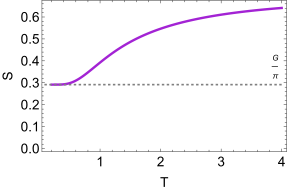
\includegraphics[width=1\linewidth]{Pictures/catalanS.eps} \\ а)}
	\end{minipage}
	\hfill
	\begin{minipage}[h]{0.5\linewidth}
		\center{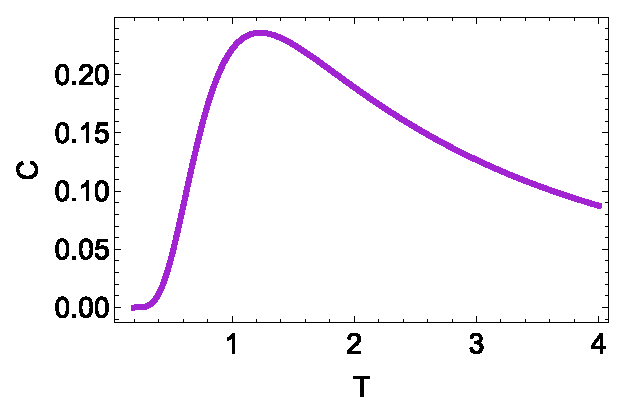
\includegraphics[width=1\linewidth]{Pictures/catalanC.eps} \\ б)}
	\end{minipage}
	\caption{Температурные зависимости обобщенной квадратной решетки c одним ферромагнитным (или антиферромагнитным) взаимодействием и тремя антиферромагнитными (или ферромагнитными) взаимодействиями: а) энтропия, б) теплоемкость. Пунктирной линией обозначена нуль-температурная энтропия: $S_{T\rightarrow 0} = G/\pi\approx 0.29156$, где $G$ --- постоянная Каталана.}
	\label{Catalan}
\end{figure}

При таком выборе знаков обменных взаимодействий спины на квадратной решетке уже не могут удовлетворить всем взаимодействиям, возникает фрустрация, а энтропия при стремлении температуры к нулю оказывается не равной нулю (рис. \ref{Catalan}а), а теплоемкость вместо острого онзагеровского пика принимает куполообразный вид (рис. \ref{Catalan}б). Значение нуль-температурной энтропии было найдено и оно выражается в виде частного двух математических констант
\begin{equation}
S_{T\rightarrow 0} = \frac{G}{\pi} = 0.29156\dots,
\label{g}
\end{equation} 
где $G$ --- постоянная Каталана, важнейшая константа в теории чисел и в комбинаторике.

Занулим теперь одно из четырех обменных взаимодействий. Пусть $J_4 = 0$, но как и прежде будем рассматривать вариант cо взаимодействиями равными единице, $|J_1| = |J_2| = |J_3| = 1$. В таком случае получается 8 вариантов выбрать знаки у взаимодействий между спинами.

\begin{align*}
	&1) +\;+\;+\;0, \qquad   5) -\;+\;+\;0, \\
	&2) +\;+\;-\;0, \qquad  6) -\;+\;-\;0, \\
	&3) +\;-\;+\;0, \qquad  7) -\;-\;+\;0, \\
	&4) +\;-\;-\;0, \qquad  8) -\;-\;-\;0.
\end{align*}

Когда мы зануляем одно из взаимодействий на обобщенной квадратной решетке мы по сути получаем гексагональную решетку~\cite{generalizedIsing2021}. Это просто понять, взглянув на рисунок \ref{hexTranf}. Действительно, занулив одно из взаимодействий, например, $J_4$, получим сначала решетку типа кирпичная кладка, и которая, в свою очередь топологически эквивалентна гексагональной решетке. И такое действие можно проделать с любым из четырех взаимодействий на обобщенной квадратной решетке, и так же получим гексагональную решетку. Поэтому вариантов выбрать знаки взаимодействий именно 8, а не больше. 

\begin{figure}[h]
	\center{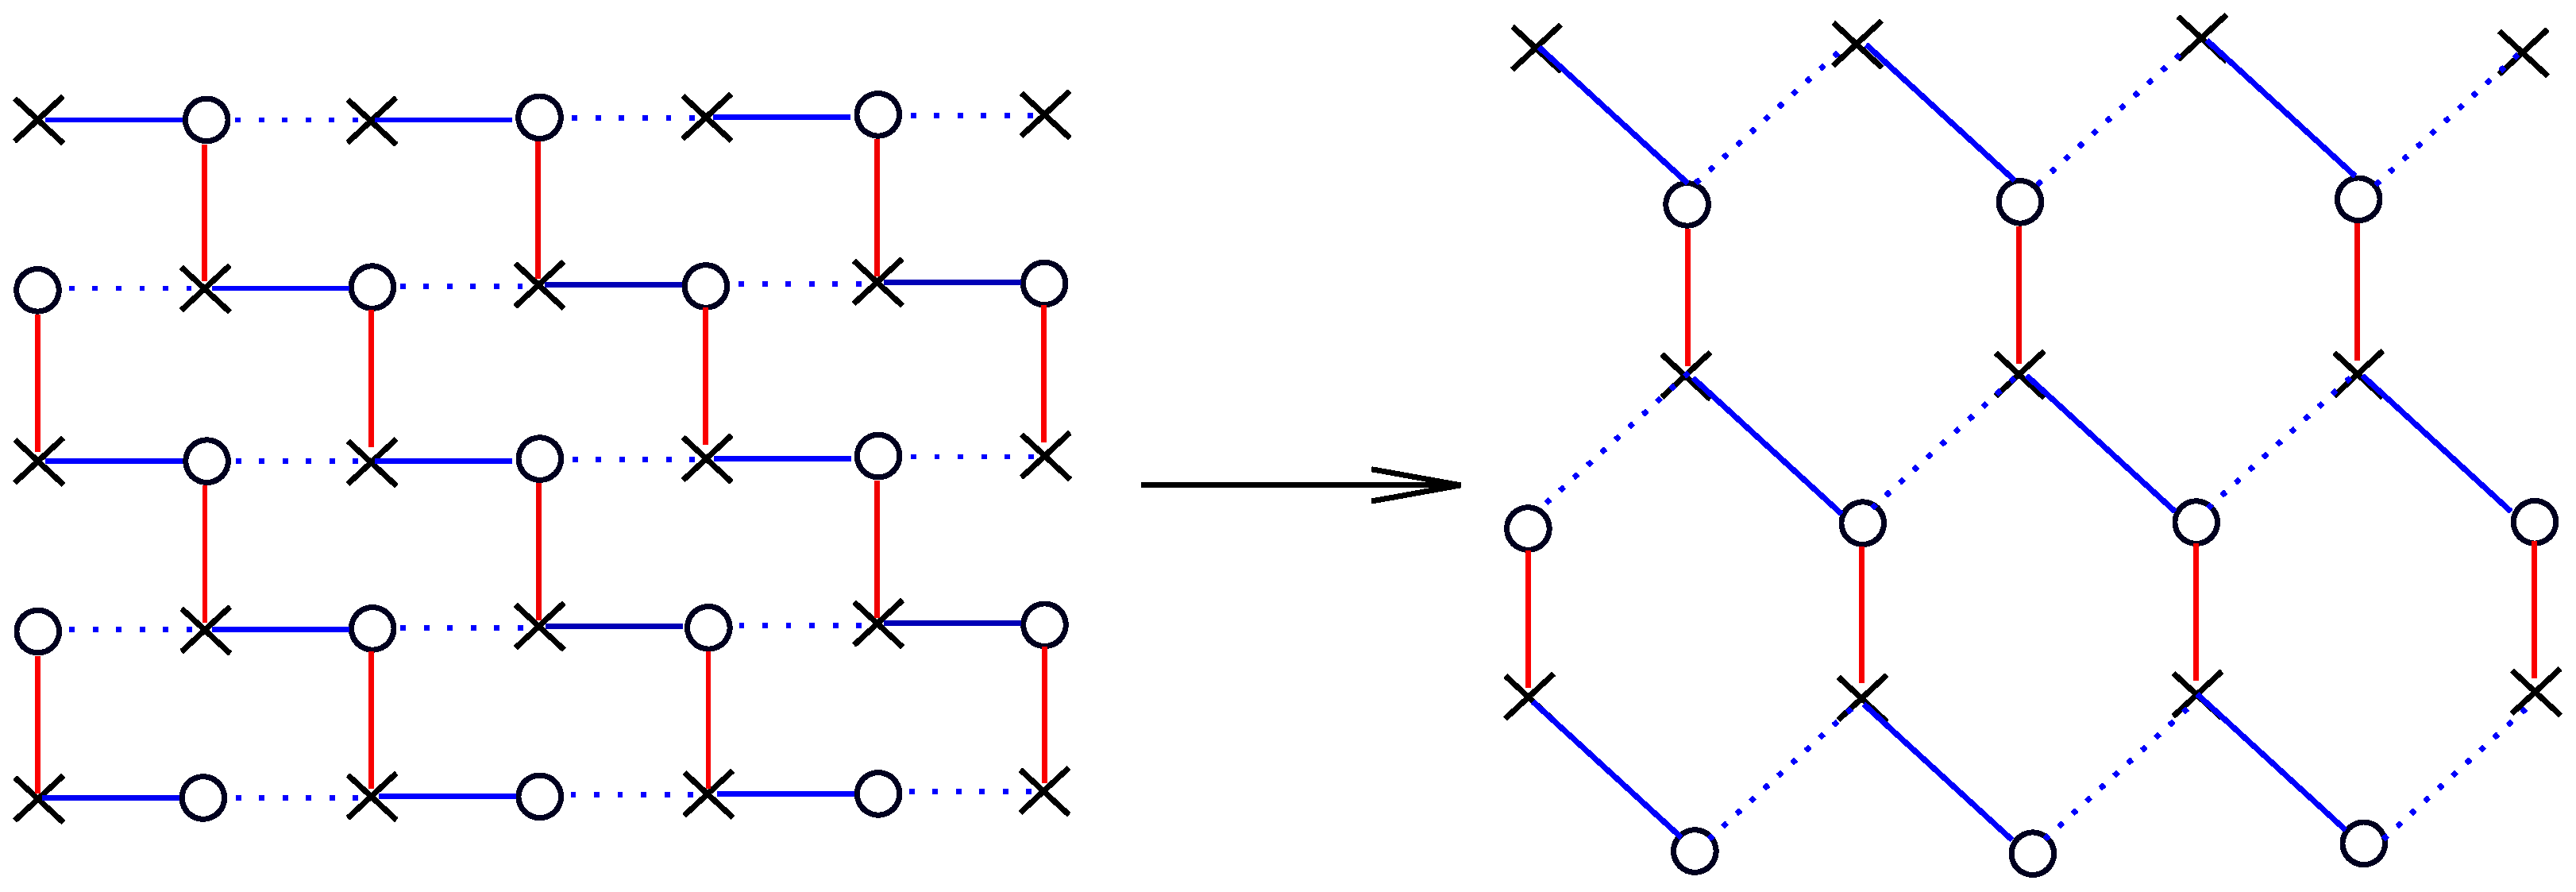
\includegraphics[width=1\linewidth]{Pictures/hex.eps}}
	\caption{При $J_4 = 0$ обобщенная квадратная решетка превращается в так называемую кирпичную кладку, которая топологически эквивалентна гексагональной решетке}
	\label{hexTranf}
\end{figure}

При исследовании вариантов выбора знаков взаимодействий, установлено, что все они дают температурные зависимости энтропии и теплоемкости, представленные на рисунке~\ref{Hex}. И это не удивительно. Ведь, как известно~\cite{houtapell1950}., гексагональная решетка при любом выборе знаков взаимодействий не имеет фрустраций.

\begin{figure}[h]
	\begin{minipage}[h]{0.5\linewidth}
		\center{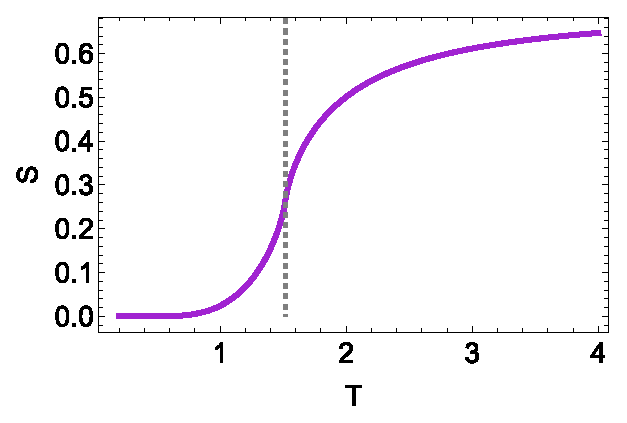
\includegraphics[width=1\linewidth]{Pictures/hexLatticeS.eps} \\ а)}
	\end{minipage}
	\hfill
	\begin{minipage}[h]{0.5\linewidth}
		\center{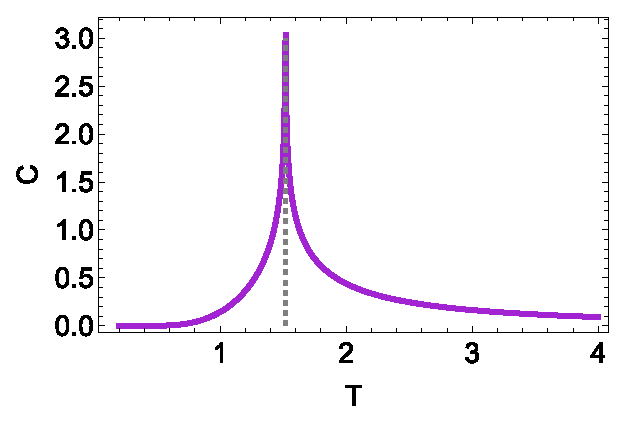
\includegraphics[width=1\linewidth]{Pictures/hexLatticeC.eps} \\ б)}
	\end{minipage}
	\caption{Температурные зависимости обобщенной квадратной решетки с тремя ненулевыми и одним нулевым взаимодействиями (гексагональная решетка): а) энтропия, б) теплоемкость. Пунктирной линией обозначена температура перехода гексагональной решетки: $T_c = 2/(\ln(2+\sqrt{3}))\approx 1.5187$.}
	\label{Hex}
\end{figure}

\begin{figure}[h]
	\begin{minipage}{0.45\linewidth}
		\center{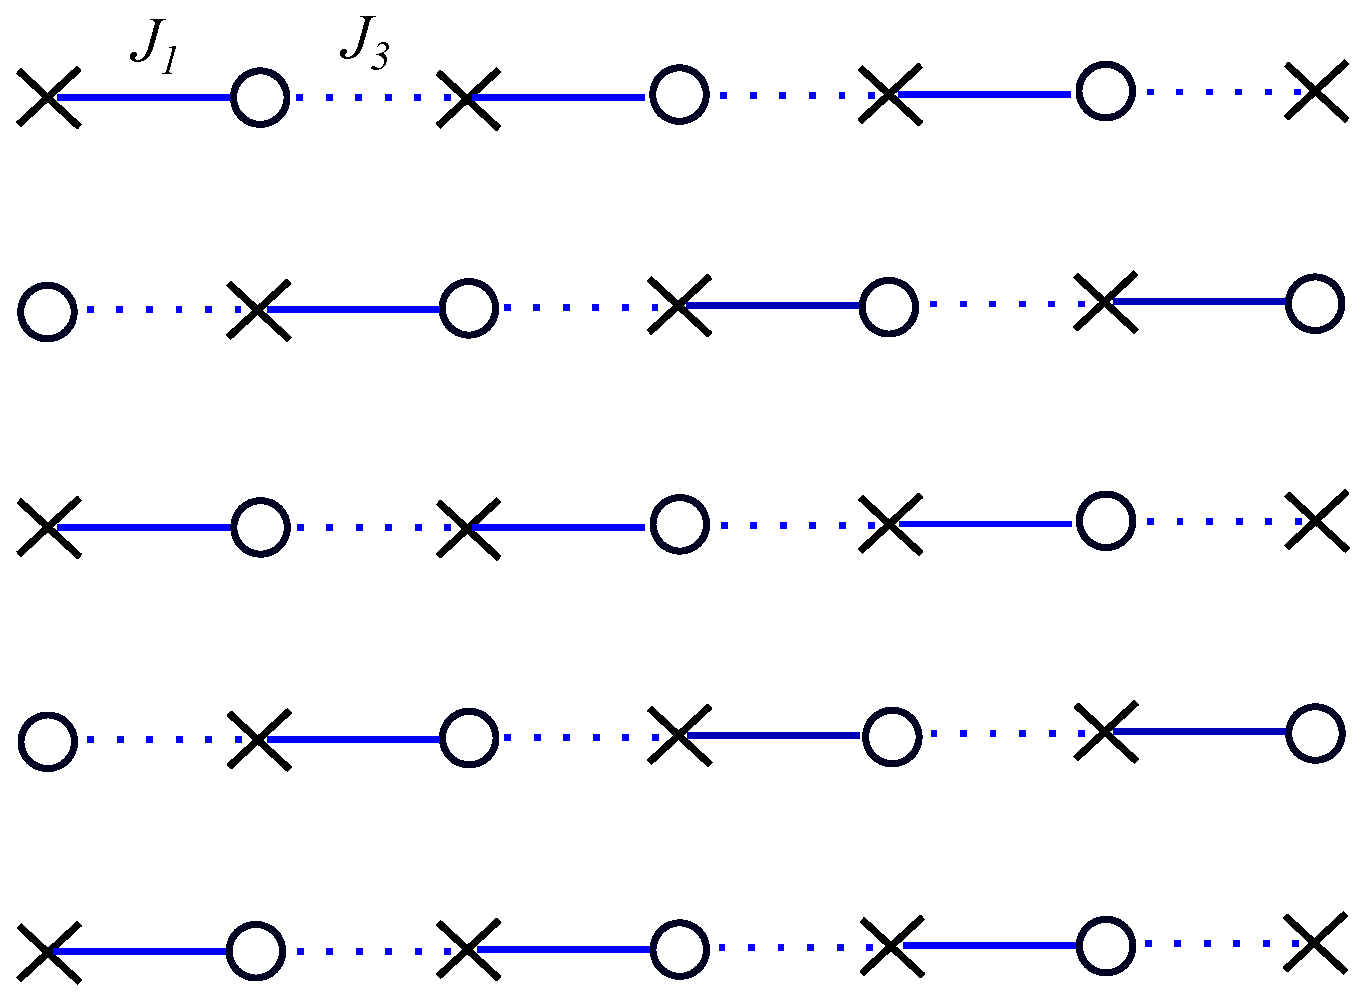
\includegraphics[width=1\linewidth]{Pictures/linear1.eps} \\ а)}
	\end{minipage}
	\hfill
	\begin{minipage}{0.45\linewidth}
		\center{\includegraphics[width=1\linewidth]{Pictures/linear2.eps} \\ б)}
	\end{minipage}
	\vfill
	\begin{minipage}{0.45\linewidth}
		\center{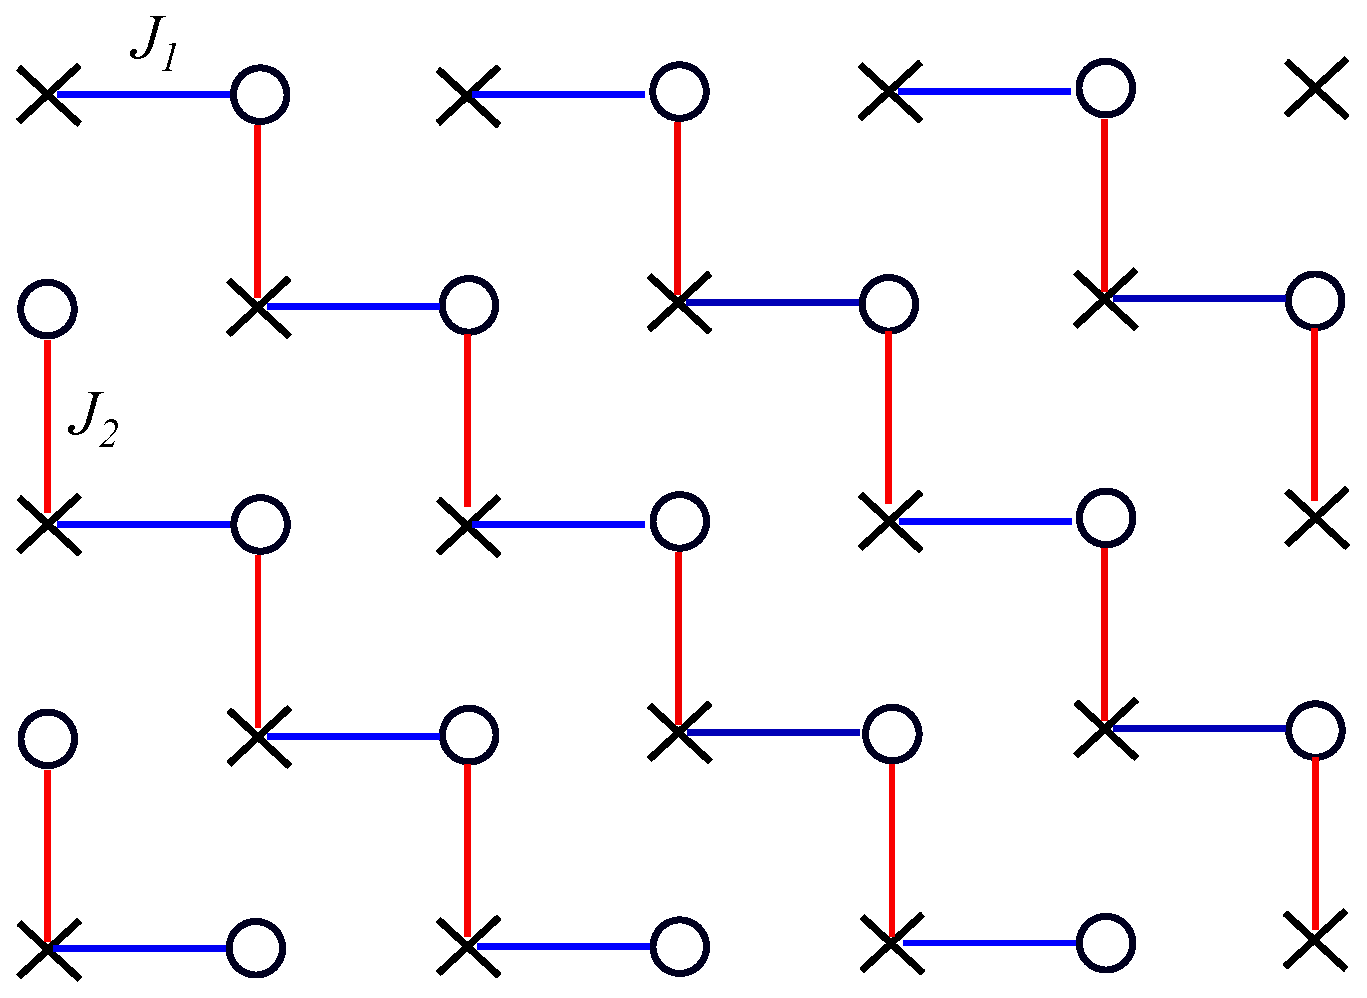
\includegraphics[width=1\linewidth]{Pictures/linear3.eps} \\ в)}
	\end{minipage}
	\hfill
	\begin{minipage}{0.45\linewidth}
		\center{\includegraphics[width=1\linewidth]{Pictures/linear4.eps} \\ г)}	
	\end{minipage}
	\caption{а) и б) "Прямые" цепочки, в) и г) Цепочки "лестничного" типа.}
	\label{linearChains}
\end{figure}

Положив равным нулю сразу два обменных взаимодействия на обобщенной квадратной решетке получим линейную цепочку. Причем, эти цепочки можно получить разных видов. Так называемые "прямые" цепочки (рис.~\ref{linearChains}а и рис.~\ref{linearChains}б) и цепочки "лестничного" типа (рис.~\ref{linearChains}в и рис.~\ref{linearChains}г). Однако, все эти цепочки показывают одни и те же температурные зависимости энтропии и теплоемкости (рис.~\ref{Linear}). И, как известно~\cite{mussardo2010}, любая линейная цепочка не обнаруживает точки перехода, кроме $T=0$.

\begin{figure}[h]
	\begin{minipage}[h]{0.5\linewidth}
		\center{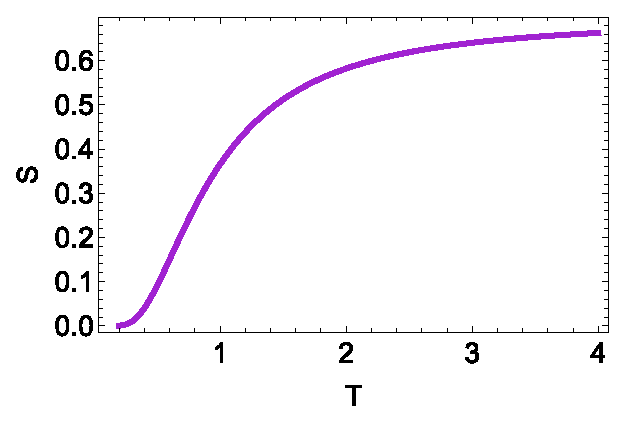
\includegraphics[width=1\linewidth]{Pictures/linearS.eps} \\ а)}
	\end{minipage}
	\hfill
	\begin{minipage}[h]{0.5\linewidth}
		\center{\includegraphics[width=1\linewidth]{Pictures/linearC.eps} \\ б)}
	\end{minipage}
	\caption{Температурные зависимости обобщенной квадратной решетки с двумя ненулевыми и двумя нулевыми взаимодействиями (линейная цепочка): а) энтропия, б) теплоемкость.}
	\label{Linear}
\end{figure}

Осталось рассмотреть случай зануления сразу трех взаимодействий из четырех, например, $J_2 = J_3 = J_4 = 0$. При таком выборе обменных взаимодействий получается решетка димеров, которая к тому же является фрустрированной. Нуль-температурная энтропия равна $\ln 2/2$.

\begin{figure}[h]
	\center{\includegraphics[width=0.45\linewidth]{Pictures/dimers.eps}}
	\caption{Решетка димеров, получаемая из обобщенной квадратной решетки, занулением любых трех взаимодействий, здесь $J_2 = J_3 = J_4 = 0$.}
	\label{dimerLattice}
\end{figure}

Взаимодействие между спинами в одном димере может быть либо ферромагнитным (спины параллельны), либо антиферромагнитным (спины антипараллельны). Таких пар, связанных спинов получается $N/2$, отсюда и двойка в знаменателе нуль-температурной энтропии. А так как пары спинов никак не влияют друг на друга, то направление спинов любой такой пары может не совпадать с направлением спинов соседних пар. Температурные зависимости энтропии и теплоемкости представлены на рисунке~\ref{Dimers}. Такие же зависимости получаются при занулении любых трех взаимодействий на обобщенной квадратной решетке вне зависимости от знака оставшегося взаимодействия (антиферромагнитное или ферромагнитное).

\begin{figure}[h]
	\begin{minipage}[h]{0.5\linewidth}
		\center{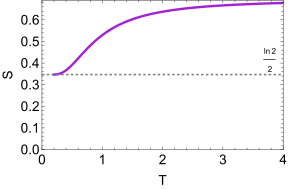
\includegraphics[width=1\linewidth]{Pictures/dimersS.eps} \\ а)}
	\end{minipage}
	\hfill
	\begin{minipage}[h]{0.5\linewidth}
		\center{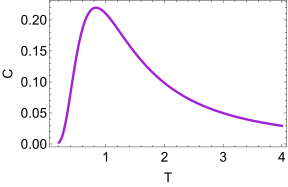
\includegraphics[width=1\linewidth]{Pictures/dimersC.eps} \\ б)}
	\end{minipage}
	\caption{Температурные зависимости обобщенной квадратной решетки с тремя нулевыми и одним ненулевым взаимодействиями (решетка димеров): а) энтропия, б) теплоемкость. Пунктирной линией обозначена нуль-температурная энтропия: $S_{T\rightarrow 0} = \ln 2/2\approx 0.34657$.}
	\label{Dimers}
\end{figure}

Наконец, когда сразу все взаимодействия равны нулю $J_1 = J_2 = J_3 = J_4 = 0$, то получаем, что энтропия вне зависимости от температуры всегда будет равна одну и тому же значению, $\ln 2$. Поскольку мы изначально рассматриваем энтропию на один узел решетки $S/N$, этот результат неудивителен и означает, что каждый спин в решетке может принимать два значения (спин вверх или спин вниз). Так как в решетке уже нет взаимодействия между спинами, то спины свободны и могут ориентироваться случайно. Это состояние в системе называется парамагнитным. Именно это состояние системы мы получаем, когда устремляем температуру к бесконечности. 

Вернемся к рассмотрению четырех ненулевых обменных взаимодействий на обобщенной квадратной решетке, а именно к случаю $J_1 = -1, J_2 = -1, J_3 = -1, J_4 = 1$ (или $J_1 = 1, J_2 = 1, J_3 = 1, J_4 = -1$). Уже известно, что при таком выборе параметров обменного взаимодействия решетка будет фрустрированной с нуль-температурной энтропией равной $G/\pi$ (рис.~\ref{Catalan}). 

Начнем увеличивать ферромагнитное значение $J_4$, а остальные взаимодействия останутся прежними. Температурные зависимости энтропий для некоторых значений обменных взаимодействий проиллюстрированы на рисунке~\ref{Peak}. При этом видно, что приведенные температурные зависимости энтропий, для которых $J_4>1$, имеют одно общее значение при $T \rightarrow 0$. 

\begin{figure}[h]
	\begin{minipage}[h]{0.5\linewidth}
		\center{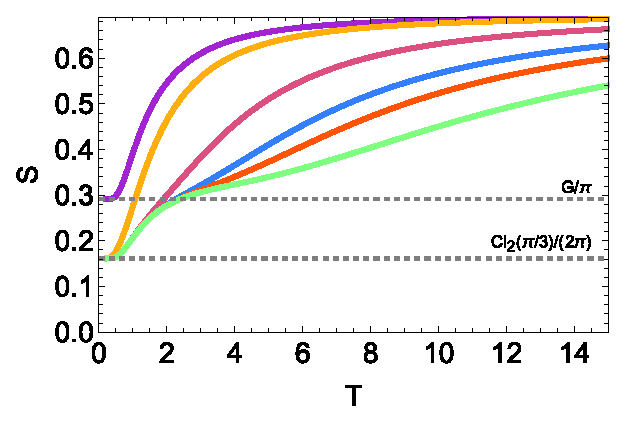
\includegraphics[width=1\linewidth]{Pictures/peakS.eps} \\ а)}
	\end{minipage}
	\hfill
	\begin{minipage}[h]{0.5\linewidth}
		\center{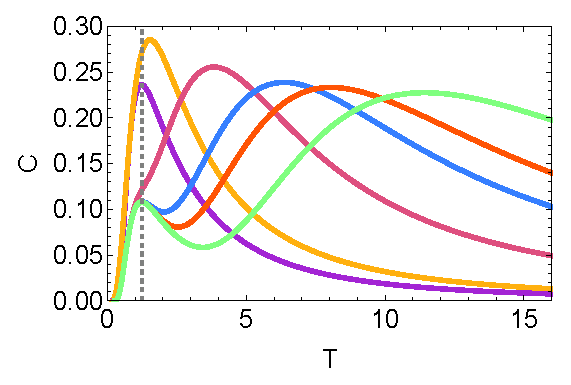
\includegraphics[width=1\linewidth]{Pictures/peakC.eps} \\ б)}
	\end{minipage}
	\caption{Температурные зависимости обобщенной квадратной решетки для различных параметров обменных взаимодействий: фиолетовая кривая --- $J_1 = -1$, $J_2 = -1$, $J_3 = -1$, $J_4 = 1$, желтая кривая --- $J_1 = -1$, $J_2 = -1$ , $J_3 = -1$, $J_4 = 2$, розовая кривая --- $J_1 = -1$, $J_2 = -1$ , $J_3 = -1$, $J_4 = 5$, синяя кривая --- $J_1 = -1$, $J_2 = -1$, $J_3 = -1$, $J_4 = 8$, красная кривая --- $J_1 = -1$, $J_2 = -1$ , $J_3 = -1$, $J_4 = 10$, зеленая кривая --- $J_1 = -1$, $J_2 = -1$ , $J_3 = -1$, $J_4 = 14$: а) энтропия. Пунктирными линиями обозначены значения нуль-температурных энтропий: $S_{T\rightarrow 0} = G/\pi\approx 0.29156$, где $G$ --- постоянная Каталана, $S_{T\rightarrow 0} = \frac{1}{2\pi} \Cl_2 (\frac{\pi}{3})\approx0.16153$, где $\Cl_2 (\varphi)$ --- функция Клаузена. б) теплоемкость. Пунктирной линией обозначено положение малого гладкого пика ($T_{peak}\approx1.232$). }
	\label{Peak}
\end{figure}

Установлено, что нуль-температурное значение для энтропий, когда $J_4>1$, выражается в виде    
\begin{equation}
S_{T\rightarrow 0} = \frac{1}{2\pi} \Cl_2 \bigg(\frac{\pi}{3}\bigg)   = 0.16153\dots, 
\label{cl}
\end{equation} 
где  $\Cl_2 (\varphi)$ --- функция Клаузена. Функция Клаузена --- трансцендентная специальная функция одной переменной, которая связана с мнимой частью дилогарифма $\Li_2$
\begin{equation*}
\Cl_2 (\varphi) = \im (\Li_2 (e^{i \varphi})).
\end{equation*}

Кроме того, функция Клаузена может быть записана через различные интегральные представления, которые можно найти в математическом справочниках и статьях (например, \cite{abramowitz_stegun1972, wood1968}).

Интересно то, что постоянную Каталана так же можно выразить через функцию Клаузена~\cite{wood1968}
\begin{equation*}
G = \Cl_2 \bigg(\frac{\pi}{2}\bigg) = \im (\Li_2 (i)),
\end{equation*}

\noindent поэтому фрустрационное значение энтропии в выражении \eqref{g} может быть переписано в виде
\begin{equation}
\frac{G}{\pi} = \frac{1}{\pi} \Cl_2 \bigg(\frac{\pi}{2}\bigg) = 0.29156\dots
\end{equation}

Кроме того, при увеличение ферромагнитного значения $J_4$ можно заметить нехарактерную особенность, связанную с теплоемкостью~(рис.~\ref{Peak}). Начиная со значения $J_4 = 5$ (розовая кривая на рисунке~\ref{Peak}б), формируется дополнительный гладкий пик теплоемкости, в то время как большой гладкий пик растягивается и смещается вправо. Более того положение дополнительного гладкого пика теплоемкости не меняется относительно увеличения ферромагнитного значения $J_4$, в то время как большой пик теплоемкости постоянно меняется. Что же касается энтропий, то их нуль-температурные значения при $J_4>1$ равны одному и тому же значению $\frac{1}{2\pi} \Cl_2 (\frac{\pi}{3})$. Все те же рассуждения справедливы для случая, когда $J_1 = 1, J_2 = 1, J_3 = 1$ и антиферромагнитном увеличении $J_4$.

Такое поведение необычно для фрустрированной системы, поэтому это требует дополнительного исследования.  

\begin{figure}[h]
	\begin{minipage}[h]{0.5\linewidth}
		\center{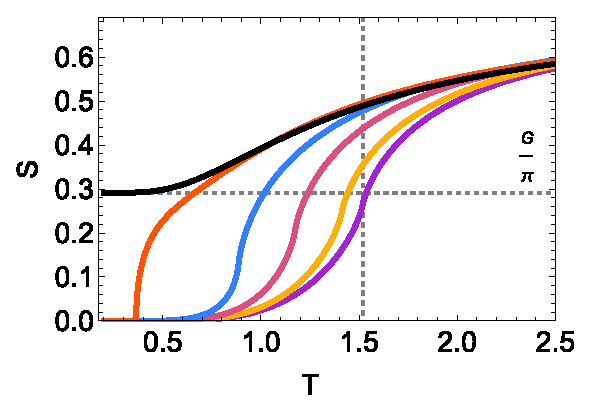
\includegraphics[width=1\linewidth]{Pictures/peak2S.eps} \\ а)}
	\end{minipage}
	\hfill
	\begin{minipage}[h]{0.5\linewidth}
		\center{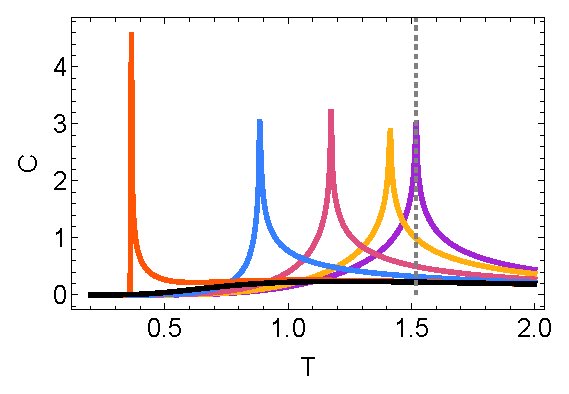
\includegraphics[width=1\linewidth]{Pictures/peak2C.eps} \\ б)}
	\end{minipage}
	\caption{Температурные зависимости обобщенной квадратной решетки для различных параметров обменных взаимодействий: фиолетовая кривая --- $J_1 = -1$, $J_2 = -1$, $J_3 = -1$, $J_4 = 0$, желтая кривая --- $J_1 = -1$, $J_2 = -1$ , $J_3 = -1$, $J_4 = 0.1$, розовая кривая --- $J_1 = -1$, $J_2 = -1$ , $J_3 = -1$, $J_4 = 0.3$, синяя кривая --- $J_1 = -1$, $J_2 = -1$, $J_3 = -1$, $J_4 = 0.5$, красная кривая --- $J_1 = -1$, $J_2 = -1$ , $J_3 = -1$, $J_4 = 0.8$, черная кривая --- $J_1 = -1$, $J_2 = -1$ , $J_3 = -1$, $J_4 = 1$: а) энтропия. Пунктирными линиями обозначены значение нуль-температурной энтропии: $S_{T\rightarrow 0} = G/\pi\approx 0.29156$, где $G$ --- постоянная Каталана и значение точки перехода для гексагональной решетки $T_c = 2/(\ln(2+\sqrt{3}))\approx 1.5187$. б) теплоемкость. Пунктирной линией обозначено значение точки перехода для гексагональной решетки $T_c = 2/(\ln(2+\sqrt{3}))\approx 1.5187$. }
	\label{Peak2}
\end{figure}

Рассмотрим поведение системы при приближении к точке фрустрации с обменными взаимодействиями $J_1 = -1$, $J_2 = -1$, $J_3 = -1$, $J_4 = 1$ (черная кривая на рисунке~\ref{Peak2}). Начнем с параметров $J_1 = -1$, $J_2 = -1$, $J_3 = -1$, $J_4 = 0$. Мы уже знаем, что при таком выборе взаимодействий реализуется случай гексагональной решетки~(рис.~\ref{Hex}). Энтропия и теплоемкость гексагональной решетки изображены фиолетовой кривой на рисунках \ref{Peak2}а и \ref{Peak2}б соответственно. Будем постепенно увеличивать ферромагнитное значение параметра $J_4$ от $0$ до $1$. Глядя на рисунки \ref{Peak2}а и \ref{Peak2}б, можно сделать сразу несколько выводов. Во-первых, зависимости теплоемкостей изображены в виде $\Lambda$ -- образных пиков. Это значит, что в точках, где теплоемкость испытывает скачок, имеет место фазовый переход. Следовательно, в этих точках не наблюдается бесконечного числа конфигураций с одинаковой энергией, иначе говоря, фрустрации отсутствуют. Во-вторых, при приближении к точке фрустрации $J_1 = -1$, $J_2 = -1$, $J_3 = -1$, $J_4 = 1$ (черная кривая на рисунке~\ref{Peak2}) зависимости теплоемкостей, смещаясь влево по температуре, испытывают укручение левой части графика.

\begin{figure}[h]
	\begin{minipage}[h]{0.5\linewidth}
		\center{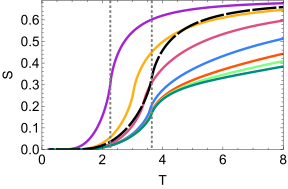
\includegraphics[width=1\linewidth]{Pictures/triangularS.eps} \\ а)}
	\end{minipage}
	\hfill
	\begin{minipage}[h]{0.5\linewidth}
		\center{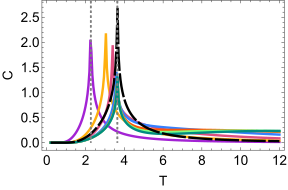
\includegraphics[width=1\linewidth]{Pictures/triangularC.eps} \\ б)}
	\end{minipage}
	\caption{Температурные зависимости обобщенной квадратной решетки для различных параметров обменных взаимодействий: фиолетовая кривая --- $J_1 = 1$, $J_2 = 1$, $J_3 = 1$, $J_4 = 1$, желтая кривая --- $J_1 = 1$, $J_2 = 1$ , $J_3 = 1$, $J_4 = 3$, розовая кривая --- $J_1 = 1$, $J_2 = 1$ , $J_3 = 1$, $J_4 = 5$, синяя кривая --- $J_1 = 1$, $J_2 = 1$, $J_3 = 1$, $J_4 = 8$, красная кривая --- $J_1 = 1$, $J_2 = 1$ , $J_3 = 1$, $J_4 = 11$, зеленая кривая --- $J_1 = 1$, $J_2 = 1$ , $J_3 = 1$, $J_4 = 13$, темно-зеленая кривая --- $J_1 = 1$, $J_2 = 1$ , $J_3 = 1$, $J_4 = 15$: а) энтропия, б) теплоемкость. Серыми пунктирными линиями обозначены значения точек перехода для квадратной и треугольной решеток соответственно: $T_c = 2/(\ln(1+\sqrt{2}))\approx 2.2692$,  $T_c = 4/\ln 3\approx 3.64096$. Черной пунктирной линией обозначены температурные зависимости энтропии и теплоемкости треугольной решетки с параметрами $J_1 = J_2 = J_3 = 1$.}
	\label{Triangular}
\end{figure}

\begin{figure}[h]
	\center{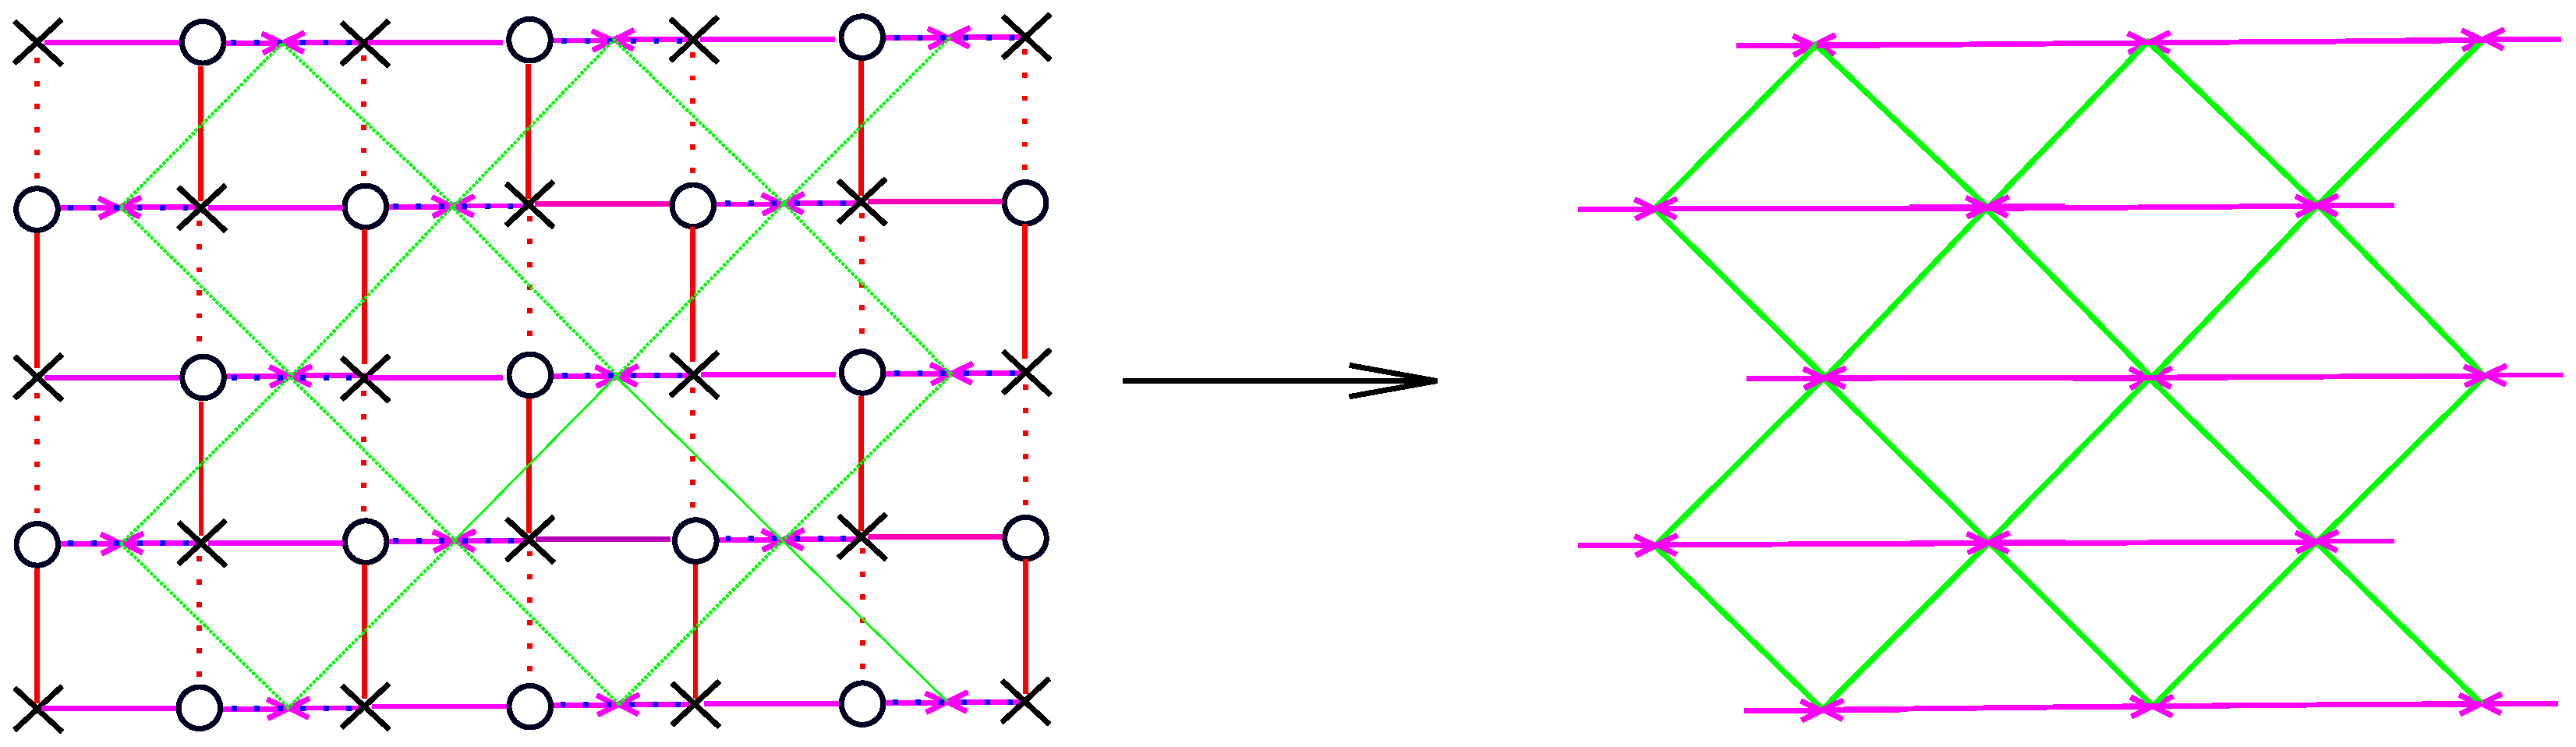
\includegraphics[width=1\linewidth]{Pictures/triag.eps}}
	\caption{Преобразование обобщенной квадратной решетки к треугольной решетке, устремляя одно из обменных взаимодействий к бесконечности}
	\label{triag}
\end{figure}

До сих пор мы не рассмотрели еще один частный случай, о котором уже ранее говорили~\cite{generalizedIsing2021}. Пусть параметры обменного взаимодействия равны $J_1 = J_2 = J_3 = J_4 = 1$ (фиолетовая кривая на рисунке~\ref{Triangular}). Этот случай уже известен и реализует обычную онзагеровскую квадратную решетку с температурой перехода $T_c = \frac{2}{\ln (1+\sqrt{2})}$~\cite{kramers_wannier1, kramers_wannier2}. При увеличении ферромагнитного взаимодействия $J_4$, энтропии и теплоемкости сходятся к некоторой точке перехода. Подтверждением этого факта служат рисунки \ref{Triangular}а и \ref{Triangular}б. Это ни что иное как температура перехода для треугольной решетки, $T_c = \frac{4}{\ln 3}$~\cite{wannier1950}. Треугольную решетку в данном случае можно получить, устремив любое из взаимодействий в бесконечность. Таким образом, обобщенная квадратная решетка сводится к треугольной решетке. Подтверждением этого является рисунок~\ref{triag}. 

Когда мы рассматривали обобщенную квадратную решетку с параметрами $J_1 = -1, J_2 =-1, J_3 = -1$ и $J_4 > 0$, происходило все то же самое. Обобщенная квадратная решетка превращалась в другую решетку под действием увеличения взаимодействия $J_4$. Но на самом деле увеличить $J_4$ мы можем только до какого-то конечного числа, а не до бесконечности. Поэтому получаем мы не треугольную решетку, а топологически искаженную решетку Кагоме~(рис.~\ref{kagomelike}). Такая решетка содержит шестиугольники и треугольники разных размеров (в отличие от обычной решетки Кагоме, в которой треугольники одного размера). 

\begin{figure}[h]
	\center{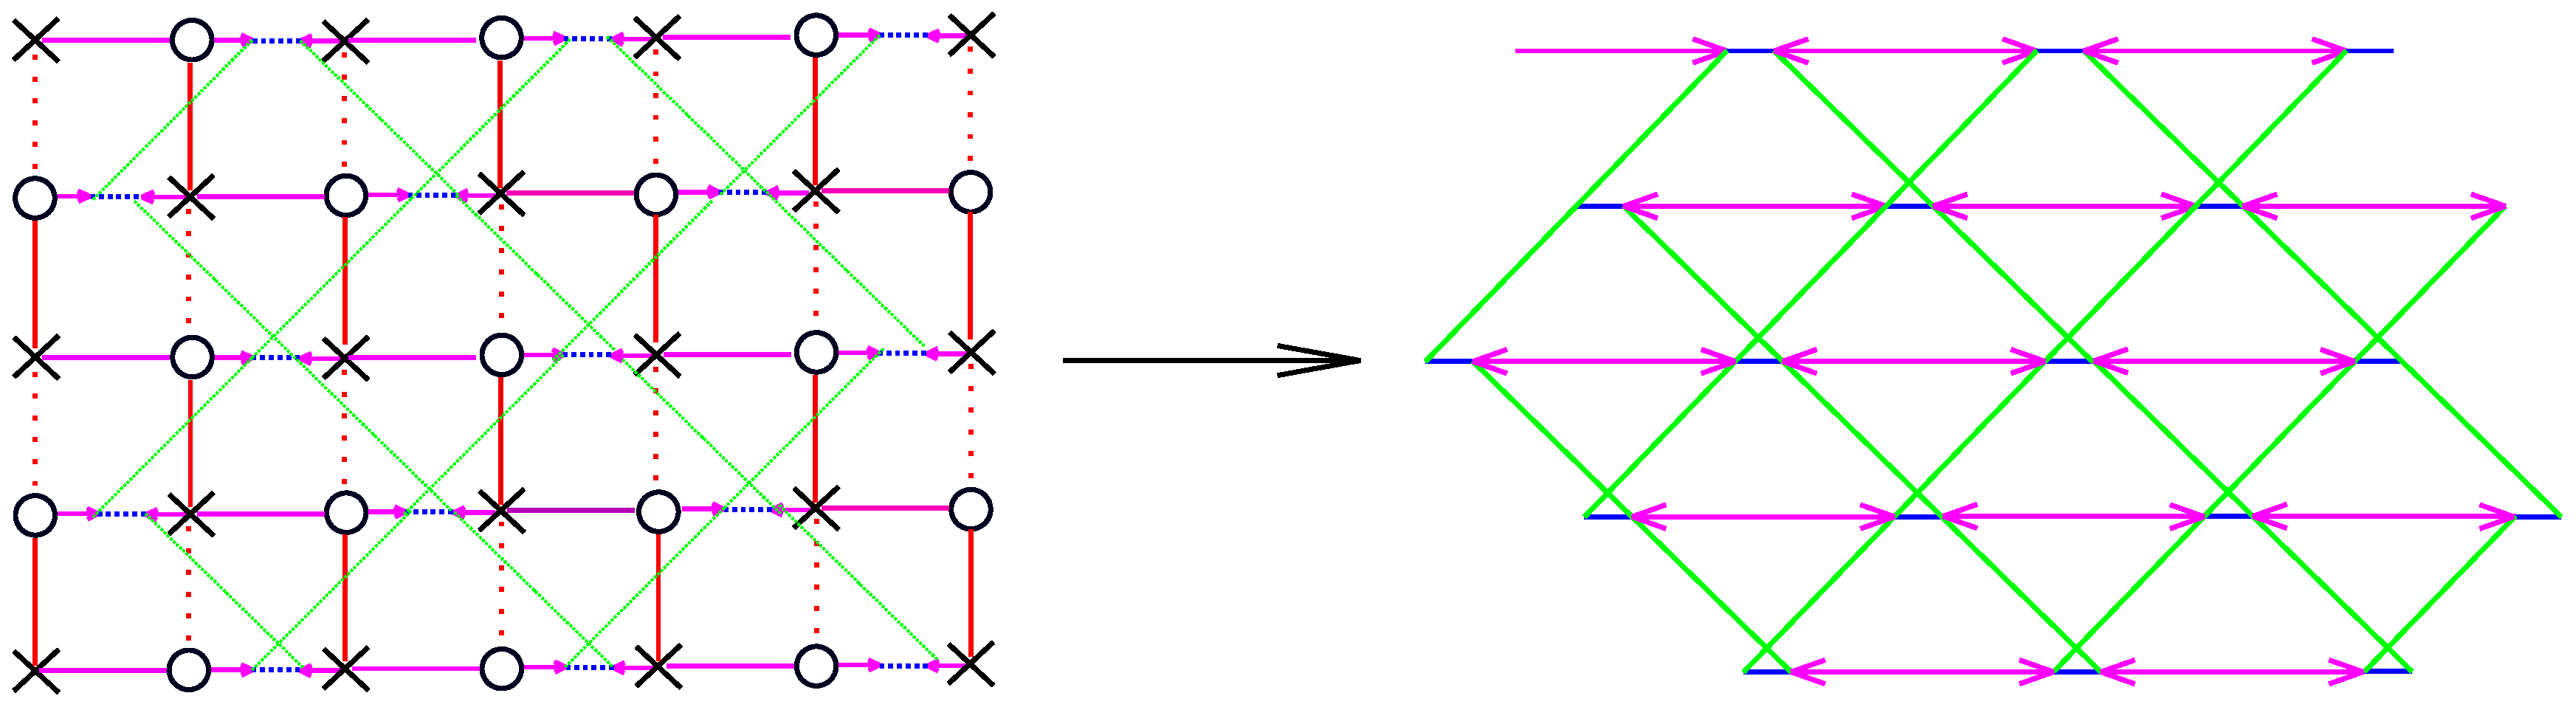
\includegraphics[width=1\linewidth]{Pictures/kagomelike.eps}}
	\caption{Получение кагоме подобной решетки из обобщенной модели Изинга при конечном увеличении одного из параметров обменного взаимодействия}
	\label{kagomelike}
\end{figure}

Напомним, что на данной решетке мы получили фрустрацию при $J_1 = -1, J_2 =-1, J_3 = -1, J_4 = 1$, а также при дальнейшем увеличении $J_4$ состояние мало того, что остается фрустрированным, так еще и все значения нуль-температурной энтропии равны одному и тому же значению $\frac{1}{2\pi} \Cl_2 (\frac{\pi}{3})$, а теплоемкость имеет дополнительный гладкий пик.

\section{Замощение шахматной решетки плитками домино}

Как упоминалось ранее, предложенная решетка Сиози~\cite{generalizedIsing2021} (по обобщению квадратной решетки на произвольное число трансляций в горизонтальном и вертикальном направлении) в самом простом случае представляется в виде так называемой шахматной решетки (с двумя трансляциями в обоих направлениях). 

Также, следует упомянуть о задаче замощения решетки плитками домино (domino tiling). Эта задача формулируется следующим образом: найти число всевозможных замощений квадратной решетки плитками домино. Эквивалентная (дуальная) задача звучит так: найти число совершенных паросочетаний на графе, в котором каждая вершина графа соответствует ячейке квадратной решетки, а ребро соответствует смежным друг с другом ячейкам решетки. И такая нетривиальная задача была решена еще в 60-x годах прошлого века Кастелайном~\cite{kasteleyn1961} и Фишером совместно с Темперли~\cite{temperley1961}.

Из данных работ следует отметить два факта. Первое --- это формула Кастелайна для числа замощений решетки плитками домино (или числа соврешенных паросочетаний на графе)~\cite{kasteleyn1961}. Эта формула работает для четных $m$ и $n$, а для нечетных значений $m$ и $n$ дает нулевое значение, что логично -- решетку с нечетным количеством квадратов на любой из сторон невозможно полностью покрыть плитками домино. 

Второе --- это асимптотическое значение, полученной формулы для бесконечных значений $m$ и $n$. Поскольку число замощений решетки при увеличении $m$ и $n$ будет тоже расти это не даст какой-либо полезной информации. Поэтому следует отыскать количество замощений квадратной решетки, приходящихся на одну плитку домино (или на один димер). Это значение было найдено авторами независимо и оно оказалось равно $\exp{(2G/\pi)}$, где $G$ -- постоянная Каталана.

В данной работе получено фрустрационное значение энтропии, приходящееся на один спин квадратной решетки, обобщенной в двух направлениях, $G/\pi$. 

Кроме того, оказалось, что еще одно значение фрустрационной энтропии, полученное в этой работе, $\frac{1}{2\pi} \Cl_2 (\frac{\pi}{3})$ ровно в два раза меньше, чем значение фрустрационной энтропии, полученное Ваннье в работе по треугольной решетке~\cite{wannier1950}, $\Cl_2 (\frac{\pi}{3}) = 0.3230\dots$.  

Все эти факты, свидетельствуют о том, что значения фрустраций энтропии в модели Изинга каким-то образом связаны с задачей о замощении решетки плитками домино. Правда этот тезис подлежит дальнейшей проверке и тщательному обоснованию.

%Нечто похожее наблюдали авторы статьи~\cite{2022}, исследуя наночастицы с ферромагнитными взаимодействиями на кагоме подобной решетке. Правда, у них в работе еще применялось внешнее магнитное поле и анизотропия. Однако, качественное совпадение теплоемкости при некоторых параметрах с полученной нами теплоемкостью с двумя горбами очевидно~(рис.~\ref{article2022}). 
%
%\begin{figure}[h]
%	\begin{minipage}[h]{0.5\linewidth}
%	\center{\includegraphics[width=1\linewidth]{New/pic1.eps} \\ а)}
%\end{minipage}
%\hfill
%\begin{minipage}[h]{0.5\linewidth}
%	\center{\includegraphics[width=1\linewidth]{New/pic2.eps} \\ б)}
%\end{minipage}
%	\caption{Теплоемкость, полученная авторами статьи~\cite{2022}, наночастиц с ферромагнитными взаимодействиями на кагоме подобной решетке.}
%	\label{article2022}
%\end{figure}

\section{Заключение}
		
Таким образом, в настоящей работе впервые получено точное аналитическое решение обобщенной модели Изинга с двумя трансляциями в горизонтальном и вертикальном направлениях на квадратной решетке комбинаторным методом Вдовиченко-Фейнмана. Исследованы термодинамические и фрустрационные свойства обобщенной модели Изинга на квадратной решетке. Исследование фрустрационных состояний показало, что при некоторых значениях и знаках обменных взаимодействий происходит расщепление теплоемкости на два гладких горба. При этом установлено, что возникающий малый горб теплоемкости никак не изменяется при бесконечном увеличении (по модулю) одного из взаимодействий. Найдены значения нуль-температурных энтропий, которые выражаются через постоянную Каталана, которая играет особую роль в теории чисел, и через так называемую функцию Клаузена. Исследованы множественные частные случаи обобщенной модели Изинга на квадратной решетке.

В заключении данной работы следует сказать, что обобщенная модель Изинга позволяет исследовать и изучать как целое многообразие новых еще неизведанных решеток, так и решетки, которые давно известны, но до сих приковывают взгляды ученых по всему миру.
		
Работа выполнена в рамках государственного задания Министерства науки и высшего образования РФ (тема «Квант», No АААА-А18-118020190095-4) при частичной поддержке Уральского отделения Российской академии наук (проект No 18-2-2-11).
	
%========================================================================
	
\begin{references}

\bibitem{ising1925} E.~Ising, Zeitschrift für Physik \textbf{21}, 253 (1925).
\bibitem{peierls1936} R.~Peierls, Proc. Cambridge Phil. Soc., \textbf{32}, 477 (1936).
\bibitem{kramers_wannier1}  H.A.~Kramers, G.H.~Wannier, Phys. Rev. \textbf{60}, 252 (1941).
\bibitem{kramers_wannier2}  H.A.~Kramers, G.H.~Wannier, Phys. Rev. \textbf{60}, 263 (1941).
\bibitem{onsager1941}  L.~Onsager, Phys. Rev. \textbf{65}, 117 (1944).
\bibitem{kac1952} M.~Kac, J.C.~Ward, Phys. Rev. \textbf{88}, 1332 (1952).
\bibitem{potts1955} R.B.~Potts, J.C.~Ward, Prog. Theor. Phys. \textbf{13}, 38 (1955).
\bibitem{hurst1960} C.A.~Hurst, H.S.~Green, J. Chem. Phys. \textbf{33}, 1059 (1960).
\bibitem{vdovichenko1964} N.V.~Vdovichenko, ЖЭТФ \textbf{47}, 715 (1964).
\bibitem{vdovichenko1965} N.V.~Vdovichenko, ЖЭТФ \textbf{48}, 526 (1965).
\bibitem{feynman1972} R.P.~Feynman, Statistical Mechanics. A Set of Lectures. Addison-Wesley, Reading, MA, (1972).
\bibitem{samuel1980} S.~Samuel, J. Math. Phys. \textbf{21}, 2015 (1980).
\bibitem{plechko1985} В.Н.~Плечко, ТМФ, \textbf{64}, 150 (1985).
\bibitem{vergeles2009} С.Н.~Вергелес, ЖЭТФ \textbf{135}, 820 (2009).
\bibitem{grunbaum1987} B.~Grünbaum, G.C.~Shephard, Tilings and Patterns, Freeman, New York, (1987).
\bibitem{wannier1950}  G.H.~Wannier, Phys. Rev. \textbf{79}, 357 (1950).
\bibitem{houtapell1950} R.M.F.~Houtappel, Prog. Theor. Phys. \textbf{16}, 425 (1950).
\bibitem{kano_naya1953}  K.~Kanô, S.~Naya, Prog. Theor. Phys. \textbf{10}, 158 (1953).
\bibitem{lin1983} K.Y.~Lin, W.J.~Ma, J. Phys. A: Math. Gen. 16, 3895, (1983).
\bibitem{lin1985} K.Y.~Lin, W.N.~Huang, Aust. J. Phys., 38, 227, (1985).
\bibitem{vaks1965} В.Г.~Вакс, А.И.~Ларкин и Ю.Н.~Овчинников, ЖЭТФ, 49, 1180 (1965).
\bibitem{urumov2002} V.~Urumov, J. Phys. A: Math. Gen. 35 (2002) 7317.
\bibitem{holzer1990} M.~Holzer, Phys. Rev. B 42, no.16, 10570, (1990).
\bibitem{lin1988} K.Y.~Lin and S.C.~Wang, Phys. Letters A, 128, (1988).
\bibitem{oitmaa2002} J.~Oitmaa and M.~Keppert, J. Phys. A: Math. Gen. 35, L219 (2002).
\bibitem{strecka2008} J.~Strečka, L.~Čanová, Acta Phys. Pol. A 113, 457 (2008). 
\bibitem{chao1990} N.C.~Chao, F.J.~Lee and K.Y.~Lin, Int. Journal of Modern Physics B 4, No.1, 113 (1990).
\bibitem{loh2008} Y.L.~Loh, D.X.~Yao, and E.W.~Carlson, Phys. Rev. B 77, 134402 (2008).
\bibitem{chikyu1987} T.~Chikyu, M.~Suzuki, Prog. Theor. Phys. 78, (6), 1242 (1987).
\bibitem{morita1986} T.~Morita, J. Phys. A: Math. Gen. 19, 1701 (1986).
\bibitem{wu1987} F.Y.~Wu, K.Y.~Lin, J. Phys. A: Math. Gen. 20, 5737 (1987).
\bibitem{syozi1972} I.~Syozi, Transformation of Ising models, in Phase transitions and Critical Phenomena Vol. 1. Exact Results, edited by C.~Domb and M.S.~Green (Academic Press, London, 1972), pp. 270–329.
\bibitem{utiyama1951} T.~Utiyama, Prog. Theor. Phys. 6, 907 (1951).



%\bibitem{yang1952} C.N.~Yang, Phys. Rev. Vol. \textbf{85}, 808 (1952).
%\bibitem{brush1967} S.G.~Brush, Rev. Mod. Phys. \textbf{39}, 883 (1967).
%\bibitem{mussardo2010}  G.~Mussardo, Statistical field theory: An introduction to exactly solved models in statistical physics (Oxford Graduate Texts), New York: Oxford University Press Inc., (2010).
%\bibitem{kaufrman1949} B.~Kaufman, Phys. Rev. \textbf{76}, 1232 (1949).
%\bibitem{kasteleyn1963} P.W.~Kasteleyn, J. Math. Phys. \textbf{4}, 287 (1963).
%\bibitem{montroll1953} G.F.~Newell, E.W.~Montroll, Rev. Mod. Phys. \textbf{25}, 353 (1953).
%\bibitem{generalizedIsing2020} Е.С.~Цуварев, Ф.А.~Кассан-Оглы, А.И.~Прошкин, ЖЭТФ \textbf{158}, 504 (2020).
%\bibitem{generalizedIsing2021} Е.С.~Цуварев, Ф.А.~Кассан-Оглы, ЖЭТФ \textbf{160}, 232 (2021).
%\bibitem{syozi1} I.~Syozi and S.~Naya, Prog. Theor. Phys. \textbf{23}, 374 (1960).
%\bibitem{syozi2} I.~Syozi and S.~Naya, Prog. Theor. Phys. \textbf{24}, 829 (1960).
%\bibitem{vaks1966} V.G.~Vaks, A.I.~Larkin, Yu.N.~Ovchinnikov, JETP \textbf{22}, 820 (1966).
%\bibitem{chikyu1987} T.~Chikyu, M.~Suzuki, Prog. Theor. Phys. \textbf{78}, 1242 (1987).
%\bibitem{toulouse1977} G.~Toulouse, Communications on Physics, \textbf{2}, 115 (1977).
%\bibitem{vannimenus1977} J.~Vannimenus, G.~Toulouse, J. Phys. C: Solid State Phys. \textbf{10}, L537 (1977).
%\bibitem{abramowitz_stegun1972} M.~Abramowitz, A.~Stegun, Handbook of mathematical functions with formulas, graphs, and mathematical tables, Applied Mathematics Series, Washington D.C.; New York: United States Department of Commerce, National Bureau of Standards; Dover Publications (1972).
%\bibitem{wood1968} Van E.~Wood, Math. Comp. \textbf{22}, 883 (1968).
%\bibitem{kasteleyn1961} P.W.~Kasteleyn, Physica \textbf{27}, 1209 (1961).
%\bibitem{temperley1961} H.N.V.~Temperley, M.E.~Fisher, Philosophical Magazine \textbf{6}, 1061 (1961).
%\bibitem{2022} Kai-Le Shi et al, Magnetization plateaus and thermodynamic properties of a ferrimagnetic Kagome-like nanoparticle under an applied magnetic field / Kai-Le Shi, Wei Jiang and Nan Si // J Mater Sci - 2022. - 57:14905–14917.
\end{references}
	
\end{document}






